
\documentclass[a4paper]{article}
\usepackage[a4paper,top=2cm,bottom=2cm,left=2cm,right=2cm,marginparwidth=2cm]{geometry}
\usepackage{lmodern}
\usepackage{listings}
\usepackage{amsmath}
\usepackage{amssymb}
\usepackage{bm}
\usepackage{textpos} % package for the positioning
\usepackage{tcolorbox}
\usepackage{pgf, tikz}
\usepackage{url}
\usetikzlibrary{arrows, automata}

\setlength{\parindent}{0em}
\setlength{\parskip}{0.3em}

\usepackage{textcomp}
\begin{document}

\lstset{language=Python,upquote=true}

\setlength{\leftskip}{20pt}
\title{Lab 3 Exercise - Optimise it!}
\author{Jonathon Hare (jsh2@ecs.soton.ac.uk)}

\maketitle

% \begin{abstract}
% \end{abstract}
% \tableofcontents

This is the exercise that you need to work through \textbf{on your own} after completing the third lab session. You'll need to write up your results/answers/findings and submit this to ECS handin as a PDF document along with the other lab exercises near the end of the module (1 pdf document per lab). 

We expect that you should aim to use one side of A4 to cover your responses to \emph{this} exercise. This exercise is worth 5\% of your overall module grade.

\section{Exploring optimisation of analytic functions}\label{analytic}
In the lab you looked at optimising Himmelblau's Function. Now we're going to explore something even more challenging. The Rastrigin Function is a fun optimisation challenge with many local minima and a single global minima:
\center
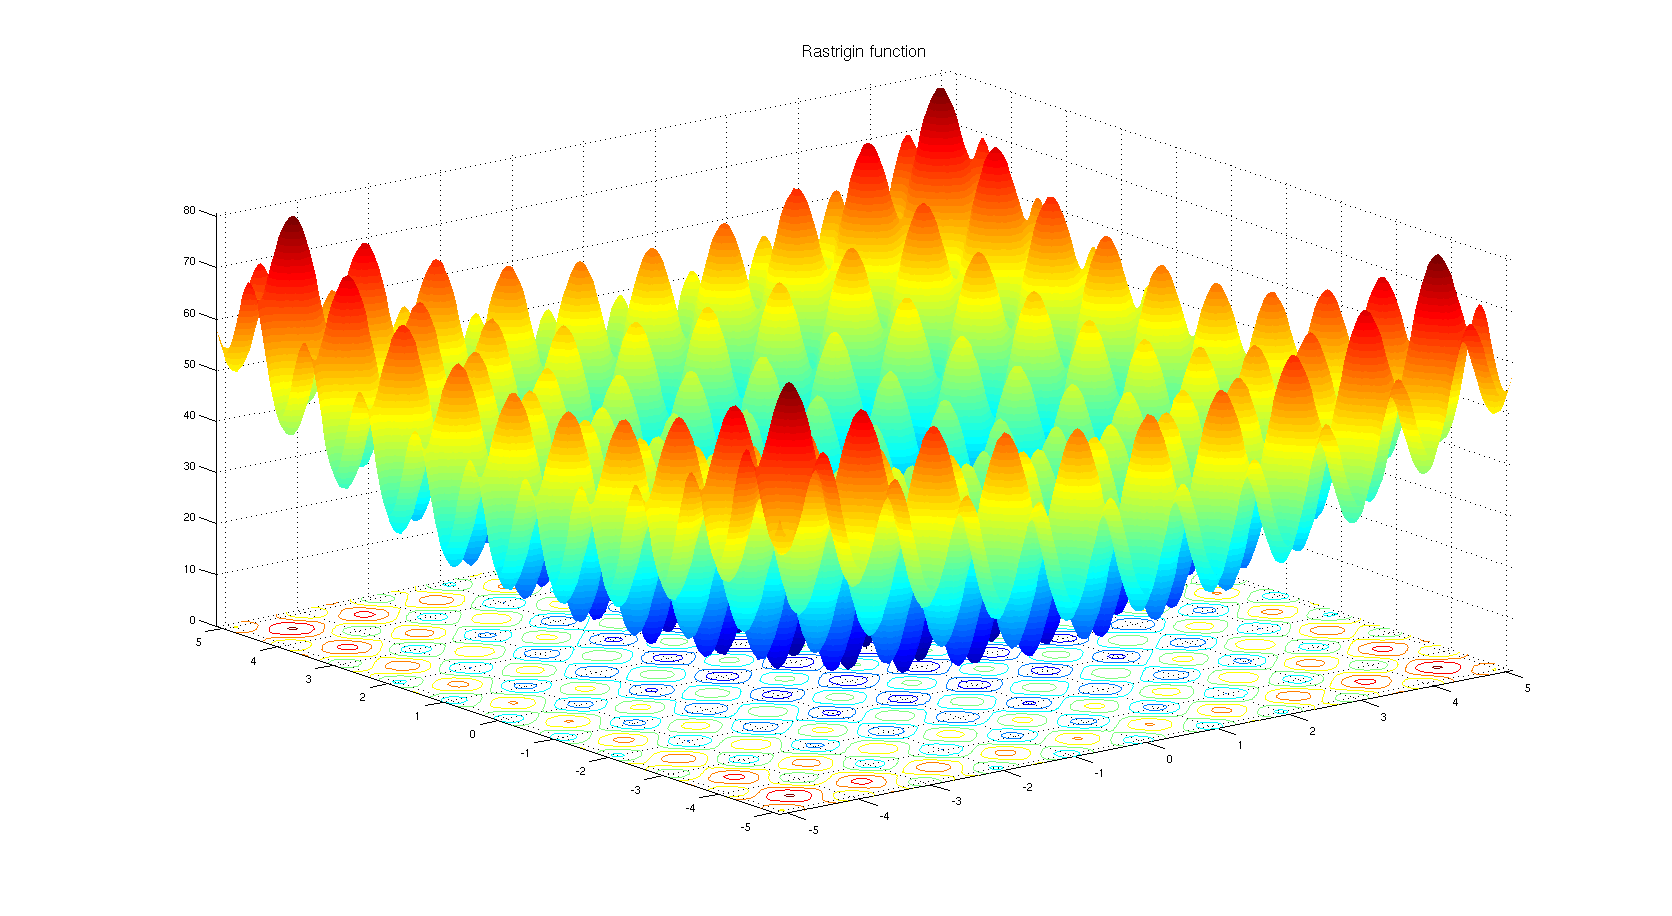
\includegraphics[width=0.8\textwidth]{Rastrigin_function.png}

\begin{tcolorbox}[title=1.1 Rastrigin (3 marks)]
Consider the 2D Rastrigin function (\url{https://en.wikipedia.org/wiki/Rastrigin\_function}). Starting at $[5, 5]$ compute the point where the following optimisers arrive at after 100 epochs:

\begin{itemize}
	\item SGD (lr=0.01)
	\item SGD+Momentum (lr=0.01, momentum=0.9)
	\item Adagrad (lr=0.01)
	\item Adam (lr=0.001)
\end{itemize}

Create a loss plot showing the function value at each epoch for each of the different optimisers. Use the PyTorch implementations of the optimisers with the default values for unspecified parameters.
\end{tcolorbox}

\section{Optimisation of a SVM on real data}\label{SVM}
The second part of the lab saw you apply a soft-margin SVM to artificially generated data and optimise its parameters with gradient descent. Now we're going to do the same with real data.


\end{document}



